\documentclass[10pt,letterpaper]{article}
\usepackage[margin=1in]{geometry}
\usepackage{newtxtext,newtxmath}
\usepackage{microtype}
\usepackage{booktabs,array,amsmath}
\usepackage{graphicx,tikz,pgfplots}
\usepgfplotslibrary{polar}
\pgfplotsset{compat=1.18}
\definecolor{cmColor}{HTML}{0072B2}
\definecolor{ppmColor}{HTML}{D55E00}
\definecolor{oTwoColor}{HTML}{CC79A7}
\definecolor{xzColor}{HTML}{444444}
\definecolor{zstdColor}{HTML}{009E73}
\usetikzlibrary{arrows.meta,positioning}
\usepackage[hidelinks]{hyperref}
\usepackage{enumitem}
\usepackage{titlesec}
\usepackage{placeins,needspace}
\renewcommand{\thesection}{\Roman{section}}
\renewcommand{\thesubsection}{\Alph{subsection}}
\renewcommand{\thesubsubsection}{\arabic{subsubsection}}
\titleformat{\section}{\centering\normalfont\normalsize\scshape}{\thesection.}{0.6em}{}
\titleformat{\subsection}{\normalfont\normalsize\itshape}{\thesubsection.}{0.6em}{}
\titleformat{\subsubsection}[runin]{\normalfont\normalsize\itshape}{\thesubsubsection)}{0.6em}{}[:]
\titlespacing*{\section}{0pt}{2.5ex plus 1ex minus .2ex}{1.3ex plus .2ex}
\titlespacing*{\subsection}{0pt}{2ex plus .5ex minus .2ex}{1ex plus .2ex}
\titlespacing*{\subsubsection}{1em}{1.5ex plus .5ex minus .2ex}{.5em}
\setlist{nosep,leftmargin=*}
\setlength{\parindent}{1em}
\setlength{\parskip}{0pt}
\setlength{\emergencystretch}{1em}
\widowpenalty=10000
\clubpenalty=10000
\renewcommand{\topfraction}{0.9}
\renewcommand{\textfraction}{0.08}
\renewcommand{\floatpagefraction}{0.8}
\hypersetup{pdftitle={Arithmetic Coding with Adaptive Context Models},
 pdfauthor={Darrell Long},
 pdfsubject={Design and evaluation of the acz file compressor},
 pdfkeywords={arithmetic coding, prediction by partial matching, context trie, context mixing, bounded memory, compression}}
\newcommand{\acz}{\texttt{acz}}
\newcommand{\arith}{\texttt{arith}}
\newcommand{\code}[1]{\texttt{#1}}
\newcommand{\MiB}{\,\mathrm{MiB}}
\input{build/metrics.tex}
\input{build/coded-command-metrics.tex}
\input{build/heldout-metrics.tex}
\begin{document}
\begin{center}
\vspace*{1em}
{\Large Arithmetic Coding with Adaptive Context Models}\\[5pt]
{\large Design and Evaluation of the \acz{} File Compressor}\\[14pt]
Darrell Long\\[5pt]
10 November 2026\\[7pt]
\textit{Dedicated to the memory of my colleague Glen G. Langdon}
\end{center}
\begin{abstract}
The \acz{} file compressor combines finite-precision arithmetic coding with adaptive byte models, prediction by partial matching (PPM), and context mixing. Its order-six PPM keeps contexts in a trie stored in two arrays, uses binary escape estimates and information inheritance based on Shkarin's published methods, and codes events with a byte-normalized multi-symbol range coder. The context mixer combines local statistics, bit histories, long matches, and record contexts in integer arithmetic. Its logistic tables are computed from the function's definition, and it finds record lengths with a sequential test on predictive code lengths. Independent blocks permit parallel coding, while optional repeat removal carries information across block boundaries. On the twelve-file Silesia corpus, with one worker per program, context mixing produces \CmMB{} MB from \InputMB{} MB of input, \CmSmallerXz\% less than \code{xz -9}, in \CmEncode{} seconds of encoding and \CmDecode{} seconds of decoding. On held-out samples of U.S. Census Bureau data (\CensusGB{}~GB) and Backblaze hard drive statistics (\BackblazeGB{}~GB), it produces \CensusCM\% and \BackblazeCM\% of input, against \CensusXz\% and \BackblazeXz\% for \mbox{\code{xz -9}}. PPM produces \PpmMB{} MB and takes \PpmEncode{} seconds to encode and \PpmDecode{} seconds to decode. Against the earlier trie model and coder in a balanced experiment, its model and coder reduce bytes by 3.46\% and encoding CPU time by 10.69\%; its output is \PpmPortLarger\% larger than that of the PPMd-H port in release 0.5.0.
\end{abstract}

\section{Introduction}
A lossless compressor models regularities in its input and assigns short representations to likely events. Arithmetic coding separates these tasks: a model supplies conditional probabilities, and the coder represents the event sequence using a length close to its cumulative information content. Changing the model can improve compression without changing the coder. This separation follows Langdon and the finite-precision implementations of Witten, Neal, and Cleary and of Moffat, Neal, and Witten~\cite{langdon,witten,moffat}.

The \arith{} library supplies the coding engines, and \acz{} divides input into independently coded blocks. Five selectable models range from byte-frequency counts to context mixing. PPM~\cite{cleary} backs off through successively shorter byte contexts, whereas the mixer combines several predictions for each bit. Both learn while coding, so neither requires a probability table in the file header.

PPM needs exact context identity to traverse its escape chain and exclude symbols already considered. \acz{} keeps its contexts in a trie whose nodes are linked to their suffixes, after Moffat~\cite{moffatppm}, stored in two arrays and addressed by index. Context mixing uses fixed tables with approximate context identity. The container delimits coded blocks, checks their integrity, bounds the number of live models, and stores incompressible blocks verbatim.

\section{Coding Engines}\label{sec:coders}
Let $x_1,\ldots,x_n$ be a sequence of model events with probabilities $0<p_i\leq1$. Its ideal code length is
\begin{equation}
  I(x_1,\ldots,x_n)=-\sum_{i=1}^n\log_2 p_i.
\end{equation}
An event can be a byte, a bit, or a PPM escape. Finite-precision coding replaces exact real intervals with integer subintervals. Encoder and decoder must use identical rounding, normalization, and model updates.

\subsection{General Interval Coder}
The general coder represents a closed interval $[L,H]$ in a 32-bit coding space. The implementation stores the endpoints and intermediate products in unsigned 64-bit integers. If an event occupies cumulative frequencies $[a,b)$ in a distribution with total $T$, let $R=H-L+1$. The update is
\begin{align}
 L' &= L+\left\lfloor\frac{Ra}{T}\right\rfloor, &
 H' &= L+\left\lfloor\frac{Rb}{T}\right\rfloor-1.\label{eq:interval}
\end{align}
Both expressions use the old $L$. The interface requires $0\leq a<b\leq T\leq 2^{30}$. Normalization leaves $R>2^{30}$ before the next event, so every positive frequency receives a nonempty interval. The largest product is at most $2^{62}$ and fits the intermediate type.

Normalization handles three cases. If the interval lies in the lower half of the coding space, the encoder emits zero. If it lies in the upper half, it emits one and subtracts $2^{31}$ from both endpoints. If it lies in the middle half, $[2^{30},3\cdot2^{30})$, the leading bit is still undecided: the encoder subtracts $2^{30}$ and increments a pending-bit count. After each case it doubles the interval, using $H\leftarrow 2H+1$ to preserve an inclusive upper endpoint. The process repeats until none of the cases applies.

Pending bits resolve the carry ambiguity without revisiting output. When a later leading bit is known, every pending bit is its complement. For example, emitting a zero after three middle-half steps emits \code{0111}. This is the standard underflow mechanism of practical arithmetic coding~\cite{witten}.

The decoder maintains a 32-bit code value inside the interval. It converts that value into a cumulative-frequency position, identifies the corresponding model event, and applies the same interval and normalization operations. Its initial read consumes 32 bits; each normalization consumes one more. To match this consumption exactly, termination emits the 32 bits of the final lower endpoint, resolving any pending bits with the first bit, then pads the last output byte with zeros. The container supplies the number of bytes to reconstruct; there is no special end-of-file symbol in the probability model. The decoder also checks the canonical end state and rejects trailing payload. Invalid intervals and I/O failures leave a coder unusable, preventing a caller from continuing from a partially updated state.

\subsection{Binary Range Coder}
A range coder is an arithmetic coder that normalizes a byte at a time; the name is Martin's~\cite{martin}. It narrows the same interval by the same rule as the coder above and differs only in the unit it shifts out. Bit models, which include all of context mixing, use a binary coder of this form with deferred carry propagation, as discussed by Moffat, Neal, and Witten~\cite[Sec.~4.2]{moffat}. Let $p_0\in(0,1)$ be the probability of zero. Its fixed-point representation is an integer $P_0\in\{1,\ldots,65535\}$, with $p_0=P_0/65536$. Given the current range $R$, the split is
\begin{equation}
  B=\left\lfloor\frac{RP_0}{65536}\right\rfloor=\lfloor Rp_0\rfloor.
\end{equation}
A zero selects the lower range of width $B$; a one advances the low endpoint by $B$ and selects width $R-B$. Before an event, normalization ensures $R\geq2^{24}$, making both choices nonempty even at the probability limits. After an event, the coder shifts out whole bytes until the invariant is restored.

A 64-bit low accumulator retains the carry above the 32-bit coding space. A carry adds one to the byte before the register and passes through any \code{0xff} bytes, so the encoder holds back the last byte below \code{0xff} and counts the \code{0xff} bytes after it. A byte that arrives with a carry releases the held byte plus one and the run as zeros; a byte below \code{0xff} without a carry releases them unchanged; a \code{0xff} joins the run. Each interval lies within the one before, so at most one carry passes any position and no written byte changes. Termination performs five byte shifts; the decoder initially reads five bytes and subsequently reads one byte per normalization. The binary interface permits byte-at-a-time normalization and event selection by one comparison. It serves the order-2 model and the context mixer; the general interval coder serves orders 0 and 1.

\subsection{Multi-Symbol Range Coder}
PPM uses a separate byte-normalized coder. Following Moffat, Neal, and Witten~\cite[Sec.~4.4]{moffat}, it first divides the range by the total, $r=\lfloor R/T\rfloor$, then advances the low endpoint by $ra$. The new width is $r(b-a)$, except for the last interval ($b=T$), which receives the remainder $R-ra$. The decoder keeps its code value relative to the low endpoint and uses two divisions: one to obtain $r$, and one to obtain a cumulative-frequency target. This differs from Equation~\eqref{eq:interval}, including its rounding order.

Before an event, $2^{48}\leq R<2^{56}$ and $T\leq2^{20}$, so $r\geq2^{28}$. Binary decisions use the upper-part probability $P_1/65536$, with $1\leq P_1<65536$, and split at $\lfloor R/65536\rfloor(65536-P_1)$. This is division before multiplication, unlike the binary coder above. Normalization shifts whole bytes and defers a carry in the same way as the binary coder. Termination writes eight bytes including the held-back byte. The decoder reads eight bytes initially, rejects an initial relative code value at or above the initial range, and requires a zero relative code value and exact payload consumption at termination. Sink errors latch the encoder into a failed state.

An independent arbitrary-integer reference with immediate output and backward carry propagation matched 165 event sequences, including every nonzero 16-bit binary probability with both outcomes and a carry through 1,024 consecutive \code{0xff} bytes. Mutation, truncation, and trailing-byte checks covered 540,369 candidates in both debug and release builds.

\section{Adaptive Probability Models}\label{sec:models}
Every model is initialized at the start of a block. Encoder and decoder update its state from the same observed bytes and bits, after using each prediction. This convention permits reconstruction from the compressed stream alone. Table~\ref{tab:models} lists the model selected by each level.

\begin{table}[htbp]
\centering
\caption{Models in \acz{}. The default is level 4. A byte context contains completed preceding bytes; a bit context additionally includes the current byte's known prefix.}\label{tab:models}
\medskip
\begin{tabular}{@{}cll@{}}
\toprule
Level & Probability model & Coding engine\\
\midrule
0 & Adaptive byte frequencies & General interval\\
1 & Byte frequencies conditioned on the preceding byte & General interval\\
2 & Binary predictions conditioned on two preceding bytes & Binary range\\
3 & Prediction by partial matching, maximum byte order 6 & Multi-symbol range\\
4 & Context mixing with matches and record contexts & Binary range\\
\bottomrule
\end{tabular}
\end{table}

\subsection{Orders 0, 1, and 2}
Order 0 counts the 256 byte values. A Fenwick tree~\cite{fenwick} stores partial sums in an array, supporting cumulative-frequency queries and updates in $O(\log \lvert\Sigma\rvert)$ steps for alphabet $\Sigma$. This avoids either scanning all 256 counts for each event or changing every later cumulative total after an observation. Each count starts at one, and an observation adds 32 to the selected count. When the total exceeds $2^{16}$, every count is halved, rounding upward. This adaptation threshold discounts older observations before the coder's $2^{30}$ limit is approached. Order 1 selects one of 256 such distributions using the preceding byte. It can distinguish, for example, letters following a space from letters following another letter, but each distribution receives fewer observations.

Order 2 codes a byte as eight binary decisions, most significant bit first. The context is the preceding two bytes together with the already known bit prefix. The prefix selects a node of a binary tree over the byte alphabet; at each node a compact adaptive estimator predicts the next bit. It starts at probability $1/2$ and moves $1/16$ of the remaining distance toward the observed outcome, with the integer increment rounded down. The stored 16-bit numerator stays in $[15,65521]$, so both outcomes remain encodable. This avoids searching a 256-symbol distribution, at the expense of eight model and coder operations per byte.

\subsection{Prediction by Partial Matching}
PPM predicts a byte from the longest preceding context, of at most six bytes, that has seen it~\cite{cleary}. The contexts are tried from longest to shortest. A context that has not seen the byte codes an escape and passes to the next shorter context, and the symbols it has seen are excluded there: the byte is none of them, so the shorter context need not leave room for them~\cite{moffatppm}. Below the order-1 contexts is an order-0 distribution over the bytes already seen in the block, and below that a uniform choice among the bytes not yet excluded.

\subsubsection{Symbol and Escape Weights}
A symbol with count $f$ has weight $2f-1$, Howard and Vitter's method D~\cite{howard}. Counts are stored in half units, $h=2f$, so a half-weight update is exact and the coding weight is $h-1$. The order-0 distribution gives escape the number of visible symbols. Higher contexts use two types of learned estimate based on Shkarin~\cite{shkarin}.

A context with one symbol and no exclusions codes a binary decision between that symbol and escape. Shkarin's Section~3.1 supplies 8,192 classes: 128 count levels, four shorter-context alphabet-size classes, and four binary flags. Our count quantizer is exact in half units below 64, then has eight levels per octave, saturated at 127. Shorter alphabets are grouped as 1, 2--3, 4--15, and 16 or more symbols. The flags record whether the previous byte's successful event had probability strictly above $1/2$, whether either of the top two bits is set in each of the previous and singleton bytes, and whether more than six successive bytes were coded without escape at probability strictly above $1/2$. The previous-event test includes order 0. On first use a class starts with escape probability $1/(f+1)$, preserving half counts. Its 16-bit estimate moves $1/64$ of the distance toward the observed outcome, using an arithmetic right shift, and is clamped to $[32,65504]/65536$.

Larger contexts learn an escape \emph{frequency} $t$, rather than a common probability, so the same class can supply different probabilities $t/(W+t)$ as its visible symbol-weight sum $W$ changes. With exclusions, 400 classes use the components of Shkarin's Section~3.3. Without exclusions, 200 classes use our selected subset of the components in Section~5.5, instead of the per-context estimator of Section~3.2. Visible alphabet sizes have 25 levels, with 25 or more saturated. The masked classes also test the alphabet increase from the child, the increase to the parent, the previous byte's top bits, and whether the context's mean count $T/(m+1)$ exceeds two. The unmasked classes test $4m>3m_{\rm parent}$, the previous byte's top bits, and the long-run flag. These quantizers and thresholds are our choices.

Shkarin motivates frequency modeling but does not specify the following update. We apply Robbins and Monro's stochastic-approximation method~\cite{robbinsmonro} to an observation we designed; the observation and its integer implementation are ours. For outcome $\delta=1$ on escape and zero on a symbol, the ideal, unrounded rule is
\begin{equation}
 t\leftarrow t+\frac{\delta(W+t)-t}{N_0}.
\end{equation}
Here $W$ is the pre-decision sum used by the coder, after exclusions. A class starts at the number of visible symbols and keeps 12 fractional bits. Its window is $N_0=\min(64,2^{1+\lceil\log_2\max(4,N)\rceil})$ for $N$ previous uses. Escape adds $W/N_0$ exactly in fixed point; a hit subtracts the fixed-point value divided by $N_0$, rounding that decrement down. The learned value stays between $1/16$ and $2^{18}$; the coder uses $\max(1,\lfloor t+1/2\rfloor)$. Only the ideal unrounded, unclamped rule has zero expected drift at $q=t/(W+t)$ for fixed $W$ and escape rate $q$. For example, $W=30$, $N_0=64$, and fixed-point value 40961 give an increment of 1920 and decrement of 640: integer drift vanishes at $q=1/4$, whereas the ideal root is $40961/163841$. Floors, caps and coding-weight rounding further distinguish the implemented estimate.

\subsubsection{Learning}
After coding, the byte is counted in the successful context and added to every longer context that escaped. Update exclusion~\cite{moffatppm} is modified in one case: the immediate shorter context also receives a half-weight increment while the successful context's \emph{pre-update} symbol count is below eight and its order is below the maximum order six, following Shkarin's Section~2.2. Our mapping uses the stored count $f$ for this cutoff; it does not test the parent's count.

When a symbol is added to a context that already holds others, its initial count uses Shkarin's equation (5), with $\tau=1/4$, generalized symbol frequency $f-1/2$, and total frequency $\sum f$. Integer arithmetic rounds the inherited count down in half units and clamps it to $[1,32]$. A new singleton context delays inheritance until it is next encountered, using its suffix parent's statistics at that time, as described at the end of Section~2.1. Pending singleton ancestors are resolved shortest first before the next coding decision, without reading that decision's input byte. For this new-context case we use the values Shkarin's Section~3.1 gives for binary contexts, $\tau=1$ and initial escape frequency one; a singleton parent passes on its own count. Applying these values here, the count mappings, rounding and bounds are explicit design choices. A context reset removes pending nodes, while the class learners survive until the next block.

When a context's total stored half count exceeds 8192, counts are halved with upward rounding and a minimum stored count of two, so symbols remain encodable. A symbol whose count passes its predecessor's moves one place forward, keeping frequent symbols near the front. Encoder and decoder perform the same inheritance, rescaling, reordering and reset operations. Independent checks compared exact model-state vectors, including exclusion stamps, over 20 streams with forced resets, stamp rollover and long rescaling sequences; the cleaned model matched its selected experimental predecessor.

\subsection{Context Mixing}
PPM chooses a sequence of contexts and backs off; context mixing asks several models for predictions at once, combines them in the log-odds domain, and learns how much to trust each one. The architecture is that of the PAQ compressors as their published descriptions give it~\cite{mahoney,knoll}.

There are eighteen mixer inputs. Directly indexed order-0 and order-1 counters provide two. Seven hashed context models---byte orders 2, 3, 4, and 6, a word context, and two sparse contexts---each provide two more: an adaptive probability and a probability learned from a bit history. A match model and a constant bias supply the last two. All byte contexts are combined with the current partial byte, so prediction remains causal within a byte.

The word context combines the preceding byte with a running hash of the current run of ASCII letters, folded to lowercase and reset on a non-letter. One sparse context combines bytes two and four positions back with the current position modulo four, the same field of the previous four-byte word. The other uses the record length described below.

An adaptive counter stores a probability and an observation count $n$. Its update moves approximately $1/(n+3.5)$ of the way toward the observed bit. Direct order-0 counters cap $n$ at 60, order-1 counters at 120, and match counters at 1023. These caps keep the learning rate positive. A hashed model instead uses the sum of its two bit-history counts as $n$, with each count capped at 63. Each observation increments the matching count and reduces the opposing count, when it exceeds two, to half its value plus one, rounding down. This is Mahoney's semi-stationary update~\cite{mahoney}: evidence against the latest outcome is discounted but kept. A learned map converts this state into a second probability. The two inputs distinguish a stable long-established tendency from a similar probability based on little or recently changing evidence.

Figure~\ref{fig:cm} shows the combination of these predictions into one probability for the next bit.

\begin{figure}[htbp]
\centering
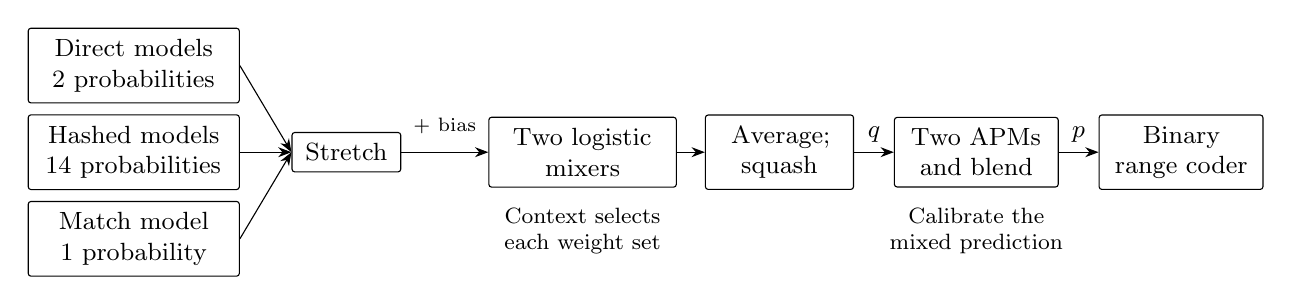
\begin{tikzpicture}[box/.style={draw,rounded corners=1pt,align=center,font=\small,inner sep=4pt},>=Stealth]
\node[box,text width=2.4cm] (direct) at (0,1.1) {Direct models\\2 probabilities};
\node[box,text width=2.4cm] (hashed) at (0,0) {Hashed models\\14 probabilities};
\node[box,text width=2.4cm] (match) at (0,-1.1) {Match model\\1 probability};
\node[box,text width=1.1cm] (stretch) at (2.7,0) {Stretch};
\node[box,text width=2.1cm] (mix) at (5.7,0) {Two logistic\\mixers};
\node[box,text width=1.6cm] (mean) at (8.2,0) {Average;\\squash};
\node[box,text width=1.8cm] (apm) at (10.7,0) {Two APMs\\and blend};
\node[box,text width=1.8cm] (coder) at (13.3,0) {Binary\\range coder};
\draw[->] (direct.east) -- (stretch.west);
\draw[->] (hashed.east) -- (stretch.west);
\draw[->] (match.east) -- (stretch.west);
\draw[->] (stretch) -- node[above=3pt,font=\scriptsize] {+ bias} (mix);
\draw[->] (mix) -- (mean);
\draw[->] (mean) -- node[above,font=\small] {$q$} (apm);
\draw[->] (apm) -- node[above,font=\small] {$p$} (coder);
\node[font=\footnotesize,align=center] at (5.7,-1.0) {Context selects\\each weight set};
\node[font=\footnotesize,align=center] at (10.7,-1.0) {Calibrate the\\mixed prediction};
\end{tikzpicture}
\caption{Context mixing for one bit. Seventeen probabilities and a constant bias become one probability through two context-dependent mixtures and two calibration maps. After coding the observed bit, the selected states and weights are trained for the next prediction.}\label{fig:cm}
\end{figure}

\subsubsection{Mixing and Calibration}
For the seventeen input probabilities $p_i\in(0,1)$, write $x_i=\ln(p_i/(1-p_i))$; the eighteenth input is the constant $x_{18}=1$. An ideal logistic mixer predicts
\begin{equation}
  q=\sigma\!\left(\sum_i w_i x_i\right),\qquad
  \sigma(z)=\frac{1}{1+e^{-z}}.
\end{equation}
For an observed bit $y$, the negative log-likelihood has weight gradient $(q-y)x_i$. The online update therefore takes the form
\begin{equation}
  w_i\leftarrow w_i+\eta x_i(y-q).
\end{equation}
This is the mixer that Knoll and de Freitas describe~\cite[Sec.~3.2]{knoll}. The implementation uses bounded integer weights and tabulates both functions, so its results are the same on every platform. Probabilities have 12 bits, and stretched values use 256 integer units per unit of log odds and lie in $[-2047,2047]$; the bias of one is stored as 256. The squash table holds
\begin{equation}
 S(d)=\min\!\left(4095,\left\lfloor\frac{4096}{1+e^{-d/256}}+\frac12\right\rfloor\right),\qquad 0\leq d\leq2047,
\end{equation}
and $S(-d)=4096-S(d)$. It is computed in integers when the program is compiled: $e^{1/256}$ is summed from its power series with 56 fractional bits, and each $e^{d/256}$ follows from the last by one multiplication. The stretch table is the discrete inverse. For each 12-bit $P$ it holds the $d$ for which $S(d)$ is nearest $P$, and among equals the $d$ nearest zero, so that $\mathrm{stretch}(4096-P)=-\mathrm{stretch}(P)$.

Two mixers use different weight selections: one is conditioned on the partial byte and four match-length classes (none, 1--15, 16--31, and 32 or more), the other on the preceding byte. Their outputs are averaged in the stretched domain.

Two adaptive probability maps then calibrate the combined prediction; this is secondary estimation~\cite[Sec.~4.2]{mahoney},~\cite[Sec.~3.1]{knoll}. For each context a map keeps a curve from input probability to output probability, as 17 knots spaced 256 units apart in the stretched domain from $-2048$ to $2048$. Equal spacing there places the knots closer together near probabilities 0 and 1, where a calibration error costs most. The curve starts as the identity. The output interpolates linearly between the two knots around the input. If the upper knot has interpolation weight $\omega\in[0,1)$, then after the bit $y$ is coded the lower knot $v_0$ and the upper knot $v_1$ move toward it in proportion to their shares,
\begin{equation}
 v_0\leftarrow v_0+\frac{(1-\omega)(y-v_0)}{64},\qquad v_1\leftarrow v_1+\frac{\omega(y-v_1)}{64},
\end{equation}
rounded to the nearest unit of 16-bit fixed point. One map is conditioned on the partial byte; the other also uses the preceding byte. The final estimate blends the mixed prediction and the two calibrated predictions with weights $1,1,2$. Let $Q,A_0,A_1$ be their 12-bit integer numerators, representing probabilities $Q/4096$, $A_0/4096$, and $A_1/4096$. The implementation computes
\begin{equation}
 P=\min\!\left(4095,\max\!\left(1,\left\lfloor\frac{Q+A_0+2A_1+2}{4}\right\rfloor\right)\right),
 \qquad p=\frac{P}{4096}.
\end{equation}
The addition of two rounds the integer average to the nearest unit. The resulting probability of a one is $p\in[1/4096,4095/4096]$, so the binary coder uses the zero-probability numerator $P_0=65536-16P$. After observing the bit, both mixers, the selected calibration points, and the context statistics are trained before the next prediction. This ordering is part of the compressed representation: changing it changes the probabilities seen by the decoder.

\subsubsection{Long Matches and Records}
The match model looks for an earlier occurrence of the recent byte suffix and predicts the continuation after a match of at least six bytes. A hash lookup supplies a candidate, which is confirmed by comparing at most 32 preceding bytes backward. An active match then grows for as long as its continuation agrees, so 32 is a confirmation limit, not a limit on the continuing match length. A counter selected by length class and expected bit turns that prediction into a probability. For length $\ell$, the counter class is $\ell$ through 15 and $\min(31,15+\lfloor(\ell-15)/3\rfloor)$ thereafter, giving finer resolution than the mixer's four classes. The history covers the entire block, allowing this model to exploit repetitions much longer than any fixed byte order. A disagreement with the predicted bits invalidates the current continuation.

Fixed-length records place related bytes a constant distance apart. One sparse model uses the bytes one and two records above the current position together with the preceding byte, and so needs the record length. A length $\ell$ is worth using if the byte $\ell$ positions back tells more about the next byte than the byte at the default distance, four, does. The detector measures this directly. Each candidate length has an adaptive model of a byte given the byte that far back, which estimates a byte seen $n$ times in $N$ occurrences of its context at $(n+1/16)/(N+16)$. The code length the model accumulates scores the candidate, as in Rissanen's predictive form of the minimum description length principle~\cite{rissanen}. Page's cumulative-sum test~\cite{page} accumulates the difference in code length between each candidate and the length in use, holding each sum at zero from below. A candidate replaces the length in use when its sum reaches 4,096 bits, and the default returns when the length in use falls that far behind it.

The candidates are the commonest gaps between a byte and the previous byte of the same value. The frequent-items algorithm of Misra and Gries~\cite{misragries} keeps eight gaps from 7 to 65,535 bytes. Each occurrence of a gap counts with the information content of its byte in whole bits, so a run of one common byte proposes nothing. A gap whose weight reaches 128 receives one of three scoring models, and gives it up when it has lost its weight and leads by nothing. The detector finds columns in fixed-width data of any kind, and the mixer still decides how much the record model is worth on each input.

\section{Context Storage and Memory}\label{sec:tables}
PPM and context mixing place different demands on their tables. A PPM context determines which symbols are excluded and how the decoder traverses the escape chain, so its identity must be exact. The mixer can tolerate collisions as loss of prediction quality, provided encoder and decoder experience the same collisions. Its tables use fingerprints and replacement to hold memory fixed.

\subsection{The PPM Context Trie}
The PPM contexts form a trie~\cite[Sec.~6.3]{knuth3}. A context is a node, and the symbols it has seen are its children. Symbol $s$ of context $c$ points to the node of $cs$, the context that follows when $s$ is coded in $c$; at the maximum order, where $cs$ would be too long, it points to $cs$ without its oldest byte. Every node also points to its suffix, the same context without its oldest byte, which is Moffat's vine pointer~\cite{moffatppm}. Figure~\ref{fig:trie} shows both kinds of link.

\begin{figure}[htbp]
\centering
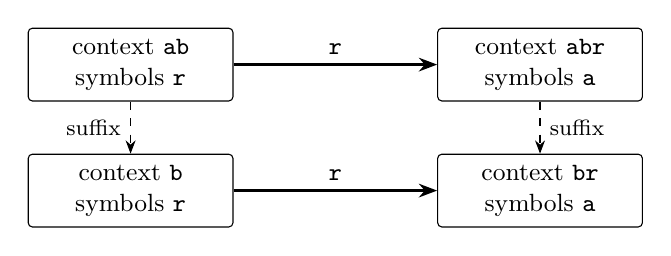
\begin{tikzpicture}[ctx/.style={draw,rounded corners=1.5pt,align=center,font=\small,inner sep=4pt,minimum width=2.6cm},>=Stealth]
\node[ctx] (ab) at (0,1.6) {context \texttt{ab}\\symbols \texttt{r}};
\node[ctx] (abr) at (5.2,1.6) {context \texttt{abr}\\symbols \texttt{a}};
\node[ctx] (b) at (0,0) {context \texttt{b}\\symbols \texttt{r}};
\node[ctx] (br) at (5.2,0) {context \texttt{br}\\symbols \texttt{a}};
\draw[->,thick] (ab) -- node[above,font=\small] {\texttt{r}} (abr);
\draw[->,thick] (b) -- node[above,font=\small] {\texttt{r}} (br);
\draw[->,dashed] (ab) -- node[left,font=\footnotesize] {suffix} (b);
\draw[->,dashed] (abr) -- node[right,font=\footnotesize] {suffix} (br);
\end{tikzpicture}
\caption{Four contexts after the text \texttt{abracadabra}. Solid arrows lead from a symbol to the context that follows it; dashed arrows from a context to its suffix. The suffix of a symbol's successor is the successor of the same symbol in the suffix, so the link from the symbol that coded a byte and the suffix links below it reach every context of the next byte.}\label{fig:trie}
\end{figure}

Coding a byte starts at the longest context and follows suffix links only as far as escapes require. Once the byte is coded, the symbol it was found as leads to the next byte's longest context. Ordinary coding therefore never searches for a context by its bytes; a table keyed by context bytes would look up as many as six contexts for each byte. Section~\ref{sec:evaluation}-\ref{sec:storage-eval} retains the comparison of the earlier estimator with both stores.

One link suffices because of a property of update exclusion: it changes how often each context counts a symbol, but not which symbols a context holds. The first time $s$ follows a context $c$, no longer context ending in $c$ can have seen $s$, so every one of them escapes and $c$ receives $s$ along with them. Hence $c$ holds $s$ exactly when the string $cs$ has occurred, and from the next byte on the context $cs$ exists and is linked from $s$. The successor of the symbol that coded a byte is thus always the longest context of the next byte. When a byte creates contexts, each is linked from the symbol that the previous byte was learned as in the context one order shorter.

Storage is bounded by restarting the model. When the next byte's updates could exceed $2^{24}$ symbol slots or 6,291,454 contexts, every context and count is discarded; the preceding bytes and the learned SEE and binary probabilities are kept, and the byte is then learned as if new. Encoder and decoder reach this decision from identical state, so no restart marker is transmitted. The contexts created at a restart are those of the current history, all at once, without the shorter contexts that would lead to them. Each is kept on a list of at most five until the symbol that leads to it is added; this list is the only place where contexts are compared by their bytes.

A node takes 12 bytes: its suffix, a link, its total count, its number of symbols, and, for a context of one symbol, that symbol, whose count is the total and whose successor is the link. A context of one symbol, the commonest kind at the longer orders, therefore needs no other storage. A context with more symbols links to an array of 8-byte slots, each holding a byte, its count, and its successor, with room for the next power of two. An array that a context outgrows goes on a free list of its size and is reused before the arena grows~\cite[Sec.~2.5]{knuth1}. Nodes and slots are addressed by 32-bit indices, so the representation does not depend on pointer width or structure layout.

For a block of $n$ bytes the model reserves $\min(2^{24},24n)$ slots and $\min(6\,291\,454,6n)+7$ nodes, the most it can use: each byte adds at most six contexts and six symbols, and a context that comes to hold $k$ symbols has taken arrays of fewer than $4k$ slots in all. At the default block size this is about 200 MiB. The arrays are reserved once and never move. A restart empties them but keeps their storage.

\subsection{Fixed Tables for Context Mixing}
Each hashed CM table is an array of 64-byte buckets. A bucket holds metadata and fifteen states, the internal nodes of a four-bit prediction tree. Looking up once per nibble supplies the states needed for four successive bit predictions, reducing hashing and memory traffic. Two adjacent candidate buckets are examined using a fingerprint. On a miss, the less-used bucket is reset for the new context; aging the other use count prevents once-frequent contexts from retaining a place indefinitely.

Fingerprints and replacement bound storage and lookup cost. A fingerprint collision can combine unrelated statistics, and replacement forgets old observations. Neither affects losslessness because both sides repeat the same operations. The fixed allocation avoids growth work in the prediction loop, while two-way lookup limits the number of candidate buckets examined.

\section{File Format and Execution}\label{sec:container}
The current format (version 14) stores independently modeled blocks, by default 16 MiB each. Figure~\ref{fig:pipeline} shows the stages. Models restart at block boundaries, allowing workers to code blocks without sharing prediction state. The writer preserves input order regardless of worker completion order.

\begin{figure}[htbp]
\centering
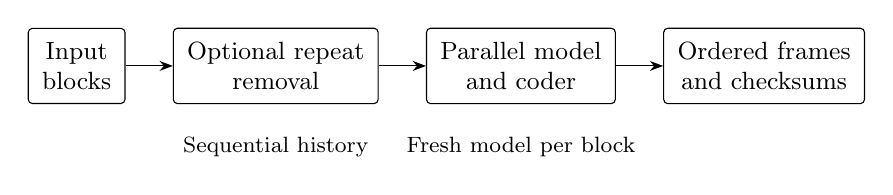
\begin{tikzpicture}[node distance=6mm, box/.style={draw,rounded corners=1.5pt,align=center,inner sep=5pt,font=\small}, >=Stealth]
\node[box] (input) {Input\\blocks};
\node[box,right=of input] (repeat) {Optional repeat\\removal};
\node[box,right=of repeat] (workers) {Parallel model\\and coder};
\node[box,right=of workers] (writer) {Ordered frames\\and checksums};
\draw[->] (input)--(repeat);
\draw[->] (repeat)--(workers);
\draw[->] (workers)--(writer);
\node[below=3mm of repeat,font=\footnotesize,align=center] {Sequential history};
\node[below=3mm of workers,font=\footnotesize,align=center] {Fresh model per block};
\end{tikzpicture}
\caption{Compression pipeline. Decoding reverses the stages: block decoding may run in parallel, while ordered reconstruction applies repeat references to the preceding output.}\label{fig:pipeline}
\end{figure}

\subsection{Framing and Error Detection}
A 16-byte file header identifies the format and model parameters. Each ordinary block has a one-byte kind, two four-byte lengths, a payload, and an eight-byte CRC-64. The checksum covers block identity and framing as well as payload. A one-byte end marker and a 16-byte trailer record the total decoded length and a CRC-64 of the reconstructed stream. These checks distinguish truncated or corrupted data from a valid arithmetic stream of the wrong length; CRCs provide error detection, not authentication.

If model coding does not reduce a block's size, the compressor stores that block verbatim. Without repeat removal, the resulting expansion bound is 17 bytes per block plus 33 bytes per file. The decoder validates lengths and kinds before allocating buffers and requires the coded payload to terminate consistently with the declared output length. Concatenated members are processed in sequence.

The command-line tool stages file output in the destination directory, flushes and synchronizes it, and publishes it only after successful completion. Without replacement permission, publication must not overwrite an existing destination; with replacement enabled, rename provides the final switch. Source removal, when requested, follows successful publication. Streaming to standard output has the usual streaming semantics: an error may follow an already written prefix.

Version 14 rejects earlier versions at each member boundary, before allocating a model. Levels 0 to 3 code the same payload as version 13; level 4 differs. Each release reads only the format it writes: version-13 files require release 0.6.0 and version-11 files release 0.5.0. Private version 12 was never released, and its number is not reused.

\subsection{Worker Admission}
The pipeline bounds the number of submitted but unfinished blocks. Completed blocks that are waiting for an earlier block still occupy a slot, so an out-of-order result queue cannot grow with the input size. Admission accounts for a model's maximum storage, rather than its smaller initial allocation. For ordinary coding with block size $B$ and model allowance $M$, the single-worker path reserves approximately $M+2B$; the parallel path reserves $M+4B$ per worker for the active, queued, and returned buffers.

At the default block size, a parallel CM worker is allowed about 213 MiB and a PPM worker about 264 MiB. A 4 GiB budget therefore admits at most nineteen CM workers or fifteen PPM workers before other options reduce the allowance. PPM reserves its arrays at block initialization; blocks of 512 KiB or less reserve less. These are storage bounds used to choose concurrency; resident memory also includes allocator and runtime overhead. On Linux, the detected budget respects every visible applicable cgroup v2 memory limit, including ancestor limits exposed through overlapping mounts; a subtree mount must not hide a tighter limit visible through a broader mount.

\subsection{Optional Long-Repeat Removal}
Independent blocks forget earlier model state. The optional \code{--dedup} stage addresses exact repetitions across those boundaries by maintaining a 256 MiB window of original input. A Karp--Rabin-style rolling fingerprint~\cite{karp} over 32 bytes samples candidate anchors, held in a direct-mapped table. Matches of at least 256 bytes become length--distance copy commands; unmatched bytes form a literal residual that is passed to the selected probability model. Differential compression similarly separates repeated regions from residual information~\cite{ajtai}.

The format stores each block's commands either as unsigned LEB128 variable-length integers~\cite[Sec.~7.6]{dwarf} or as a structured binary range code, choosing the smaller representation and adding a one-byte selector. The structured form codes the copy count, each literal run, each copy distance, each copy length less 256, and the final literal run. A number $x$ is written in Elias's gamma code~\cite{elias}: for $v=x+1$ of $n$ bits, $n-1$ in unary followed by the $n-1$ bits of $v$ below its leading one. Every bit passes through the binary coder. Each unary bit has an adaptive model for its position, the first four bits below the leading one have models chosen by $n$ and the bits before them, and the remaining bits use probability one half. Records and tables repeat at a few distances, so the four most recent distinct distances are kept in a move-to-front list~\cite{bstw}; a distance on the list is coded as its rank in unary, and any other as a number. These command models restart for each block. The decoder rejects copy counts above the block length divided by 256 before using them, then checks the reconstructed command list. The selector raises the expansion bound with repeat removal to 29 bytes per block plus 33 bytes per file.

The encoder searches only already available history. The decoder requires each copy distance $d$ to satisfy $0<d\leq\min(W,P)$, where $W$ is the window and $P$ the number of bytes reconstructed so far. Overlapping copies are valid: each copied byte refers to an earlier output position, so repeated patterns can extend beyond the original match. Reconstruction is sequential even when residual decoding runs in parallel.

Repeat removal is off by default. It adds command and history storage, and deleting a repeated span changes the adjacency seen by the statistical model. Fewer literal bytes therefore need not mean fewer compressed bytes. On Silesia it changes CM's output by less than 0.1\% in either direction (Section~\ref{sec:evaluation}-\ref{sec:coded-commands}); its value depends on the prevalence and distance of long exact repeats.

\section{Evaluation}\label{sec:evaluation}
The Silesia measurements compare compressed size and encoding and decoding CPU time across the five \acz{} models and four established compressors. Aggregate totals measure storage and computational cost for the corpus; per-file results show how the models respond to different input types. All configurations use a single worker, so these measurements do not assess parallel scaling. Section~\ref{sec:evaluation}-\ref{sec:heldout} measures compressed size on two collections not used in development.

\subsection{Method}\label{sec:method}
The evaluation uses the Silesia compression corpus~\cite{silesia}, a collection designed to test lossless compressors on varied data larger than the files in earlier benchmarks. Its twelve files include English and Polish texts, XML, source code, an application distribution, an executable, medical images, and databases. Their sizes range from 5.35 to 51.22 MB, totaling 211,938,580 bytes; Table~\ref{tab:files} identifies each file. This mixture exercises both local symbol regularities and longer repeated structures.

Each file is compressed separately, without shared history. The CPU-time experiments use the same NVIDIA DGX Spark computer, whose GB10 processor contains ten Cortex-X925 and ten Cortex-A725 CPU cores. Each process is pinned to one Cortex-X925 core, identified by Linux as logical CPU 7. Each timed configuration is run three times on that core. For each repetition, user and system CPU times are summed over all twelve files; the reported time is the median of those three sums. Every encode and decode must exit successfully, and every reconstructed file is compared byte-for-byte with its input.

The \acz{} configurations use 16 MiB blocks and one worker; both ordinary CM and CM with repeat removal are included. Comparators are XZ Utils 5.4.5 at \code{-9 -T1}, Zstandard 1.5.5 at \code{-19 -T1}, bzip2 1.0.8 at \code{-9}, and gzip 1.12 at \code{-9}. The Rust build uses rustc 1.96.0, release optimization, link-time optimization, and one code-generation unit. Sizes include file-format overhead. The retained rows, input hashes, run scripts, and build identities accompany the report; its tables are generated from those rows.

Every \acz{} row is release 0.7.0, format 14, build \code{af3e950}, timed in one run over all six configurations. The other compressors' rows come from the original experiment on the same core. As a separate reference, 7-Zip 23.01's PPMd~\cite{ppmd} was timed on the same core with order 6, a 256 MiB model, and one thread; it codes each file whole, without \acz{}'s 16 MiB blocks. Silesia was used throughout development, including model selection, and is not held out.

Level 3 was selected in run 5, which compared its five model changes and multi-symbol range coder with the earlier trie build and the PPMd-H port of release 0.5.0. Run 5 used three repetitions and a Latin-square order in which each build appears in each position twelve times across the corpus. Table~\ref{tab:current} presents all three builds. Level 3's output in release 0.7.0 has the same bytes after the header as the build timed there.



The earlier four-repetition trie-versus-hash experiment is reported in Section~\ref{sec:evaluation}-\ref{sec:storage-eval}, and the model-selection size experiments below it. A separate experiment varies only the repeat-removal threshold and measures size.

\subsection{Aggregate Compression and Time}
Table~\ref{tab:totals} reports the size of all twelve compressed files and the CPU time to encode and decode them. CM produces the smallest aggregate output: \CmBytes{} bytes, or \CmFraction\% of input. This is \CmSmallerXz\% smaller than \code{xz -9}. CM encoding takes \CmXzEncodeRatio{} times the CPU time of XZ, and decoding about \CmXzDecodeRatio{} times as much.

\begin{table}[htbp]
\centering
\caption{Silesia, sorted by compressed size. CPU seconds are medians of whole-corpus sums of user plus system time over three repetitions. Lower is better in every numeric column.}\label{tab:totals}
\medskip
\begin{tabular}{@{}lrrrr@{}}
\toprule
Configuration & Compressed bytes & \% of input & Encode (s) & Decode (s)\\
\midrule
\csname @@input\endcsname build/totals.tex
\bottomrule
\end{tabular}
\end{table}

PPM occupies an intermediate point among the \acz{} models. It produces \PpmBytes{} bytes, \PpmSmallerZstd{}\% less than \code{zstd -19}, and encodes in \PpmEncode{} seconds. Compared with CM, it is \PpmLargerCM{}\% larger but provides \PpmCMEncodeRatio{} times the encoding throughput and \PpmCMDecodeRatio{} times the decoding throughput. 7-Zip's PPMd produces \PpmRefSmaller{}\% fewer bytes and takes \PpmRefEncode{} and \PpmRefDecode{} seconds; Section~\ref{sec:evaluation}-\ref{sec:storage-eval} discusses the difference. Zstandard decodes far faster than either statistical model.

Order 2 is the fastest \acz{} encoder, taking \OTwoEncode{} seconds and producing \OTwoFraction\% of the original size. It improves both size and encoding time over the byte-oriented lower levels.

Repeat removal changes the CM total from \CmBytes{} to \DedupBytes{} bytes, an increase of \DedupLarger\%. Encoding time falls by \DedupEncodeLess\% and decoding time by \DedupDecodeLess\%, since the copied bytes bypass the model.

Figure~\ref{fig:costs} places the five configurations used in the per-file comparison on the size--time plane. CM occupies the smallest-size end, PPM lies between CM and the simple bit model in both directions, and the dictionary compressors separate strongly from both during decoding.

\begin{figure}[htbp]
\centering
\input{build/costs.tex}
\caption{Compression size versus encoding and decoding CPU time for five configurations from Table~\ref{tab:totals}. Lower and farther left is better. The horizontal axes are logarithmic; the vertical axes share a linear scale.}\label{fig:costs}
\end{figure}

\Needspace{8\baselineskip}
\subsection{Why Decoding Remains Expensive}
CM takes \CmDecode{} seconds to decode the corpus and \CmEncode{} seconds to encode it; PPM takes \PpmDecode{} and \PpmEncode{} seconds. Both directions perform adaptive modeling. The compressed stream supplies coding decisions, but it does not supply the probability distributions needed to interpret them. The decoder reconstructs those distributions from the decoded prefix and must reproduce the encoder's model updates before proceeding.

For each output byte, CM makes eight binary decisions. Each decision uses eighteen mixer inputs, two learned weighted sums, and two interpolated probability maps. After resolving the bit, the decoder updates the counters, bit histories, mixer weights, and probability maps. Hash-bucket selection is shared over four bits, but prediction and training still occur for every bit. Completing a byte also advances the match model, word context, and record detector. Thus a short code string can require substantial model work to reconstruct a long output.

PPM works at byte granularity, but a byte can require several escape decisions. The decoder follows suffix links from the longest context, computes visible symbol totals under exclusion, and searches the successful context's cumulative weights for the symbol. It then updates the successful and longer contexts, the learned escape estimates, and any new contexts and symbol arrays. The trie removes the search for contexts, but not this adaptive work.

Dictionary compressors have a different asymmetry. Their encoders search for useful matches, while their decoders receive literal and length--distance commands and reconstruct matches by copying already decoded bytes~\cite{xz,zstd}. CM's match model instead contributes a probability: it does not let the ordinary CM decoder copy an entire matched string in one step. The optional repeat-removal stage can provide such copy commands, but it has little benefit on this corpus.

Levels 3 and 4 therefore suit workloads that give compressed size substantial weight and can afford decoding CPU time. In these measurements, level 4 buys the smallest total size, while level 3 gives up some compression for \PpmCMEncodeRatio{} times the encoding throughput and \PpmCMDecodeRatio{} times the decoding throughput. A workload whose primary requirement is fast decompression is better served by a dictionary compressor.

\subsection{Variation Across Files}
Table~\ref{tab:files} gives per-file compressed fractions. CM produces the fewest bytes on every file. The aggregate in Table~\ref{tab:totals} is obtained by summing bytes, so larger files contribute proportionally more. On \code{dickens}, PPM comes within 0.04 percentage points of CM, and on \code{x-ray} it is slightly larger than order 2. The chemical database and XML file fall below 10\% of input under PPM and below 7\% under CM.

Figure~\ref{fig:kiviat} shows the compression profile of each configuration across the twelve files: the largest separation appears on some structured inputs, while the star catalog remains relatively difficult for all five.

\begin{figure}[htbp]
\centering
\input{build/kiviat.tex}
\caption{Compression across the Silesia files. Each spoke is one file; radius is compressed size as a percentage of input, from 0\% at the center to 100\% at the outer ring. Smaller radii mean better compression.}\label{fig:kiviat}
\end{figure}

\begin{table}[htbp]
\centering
\caption{Per-file compressed sizes as percentages of the original. Input sizes use decimal MB. PPM is level 3 and CM is level 4; repeat removal is disabled.}\label{tab:files}
\medskip
\small
\begin{tabular}{@{}llrrrrrr@{}}
\toprule
File & Contents & Input MB & Order 2 & PPM & CM & XZ & Zstd\\
\midrule
\csname @@input\endcsname build/files.tex
\bottomrule
\end{tabular}
\end{table}

\FloatBarrier
\subsection{Earlier Trie versus Hashed Contexts}\label{sec:storage-eval}
Before the model changes and multi-symbol coder described above, the earlier probability model was built with its contexts in a hash table, grown by linear hashing~\cite{litwin} and keyed by each context's bytes. For every byte it looks up the context of each order, and each context keeps its symbols in an array of its own. The trie build also codes each single-symbol decision with the coder's shift rather than its division, which gives the same intervals, and it allocates and reuses symbol arrays differently. The estimator and its update rules are the same, so both code the same intervals until one of them restarts; after a restart at a different byte, their states and work differ. The two builds ran alternately on the same core, four times each over the corpus, each first in two repetitions (Table~\ref{tab:storage}).

\begin{table}[htbp]
\centering
\caption{Historical run 3: the earlier PPM model with two context stores, on Silesia. These are not timings of the current estimator or coder. Times are medians of four corpus sums; peak resident memory is the largest of any one file's process.}\label{tab:storage}
\medskip
\begin{tabular}{@{}lrr@{}}
\toprule
Measure & Hash table & Trie\\
\midrule
\csname @@input\endcsname build/storage.tex
\bottomrule
\end{tabular}
\end{table}

With the trie build, encoding takes \TrieEncodeReduction{}\% less CPU time and decoding \TrieDecodeReduction{}\% less, and the maximum peak resident memory of any one process falls from \TrieRssHash{} to \TrieRss{} MiB. Of the \TreeBlocks{} blocks, \TreeQuietBlocks{} restart in neither model, and their code strings are identical. The trie uses fewer symbol slots, because a context of one symbol keeps it in its node and outgrown arrays are reused; it restarts \TreeRestarts{} times against the hash table's \TreeHashRestarts{}, and its output is \TrieBytesSaved{} bytes smaller. These figures measure the complete change: context navigation, storage and allocation, the coding of single-symbol decisions, and the restart positions that follow from them.

For the current selected level 3 in Table~\ref{tab:totals}, the separate whole-file 7-Zip PPMd reference produces \PpmRefSmaller{}\% fewer bytes, and level 3 takes \PpmRefEncodeRatio{} and \PpmRefDecodeRatio{} times its encoding and decoding time. The two differ in their estimators and memory policies as well as in \acz{}'s 16 MiB blocks.

\subsection{Selected Model and Coder}\label{sec:current}
Table~\ref{tab:current} compares the selected implementation with the preceding trie and with the historical port in run 5. The new model and coder together produce 3.456\% fewer bytes than the trie baseline and use 10.689\% less encoding CPU time and 1.874\% less decoding CPU time. Against the port they produce 2.797\% more bytes and use 21.437\% and 15.888\% more encoding and decoding CPU time. The port is \code{debc62e}, format 10. Its level-3 model and coder are those of public release 0.5.0: their sources differ only in a dedication comment. Users upgrading from 0.5.0 should therefore expect about 2.8\% larger level-3 files on this corpus at matching settings with repeat removal off.

\begin{table}[htbp]
\centering
\caption{Run 5, Silesia: the selected five model changes and multi-symbol coder (New), the preceding trie (Trie), and historical port (Port). Times are medians of three whole-corpus sums. RSS is the maximum observed peak of an individual process, not model allocation. All use 16 MiB blocks and one worker. New was timed as private format 12; format 13 was checked separately for header-only changes.}\label{tab:current}
\medskip
\small
\begin{tabular}{@{}lrrr@{}}
\toprule
Measure & New & Trie & Port\\
\midrule
\csname @@input\endcsname build/current-comparison.tex
\bottomrule
\end{tabular}
\end{table}

\subsection{Held-Out Collections}\label{sec:heldout}
Silesia guided development, so two collections of public tabular data that were not used during development measure compressed size elsewhere. The Census collection is a mirror of the U.S. Census Bureau's public data files: 996,923 files totaling 2.46 TB. Its sample is stratified over nineteen file types, among them CSV and other text files, dBase tables, Excel workbooks, SAS data sets, KML, and gzip and ZIP archives. A 152-file pilot set each type's sample size so that the type's geometric mean of the ratio of \acz{} size to \mbox{\code{xz -9}} size would be estimated within 1\% at 95\% confidence; pilot files are excluded. The Backblaze collection is Backblaze's published hard drive statistics, one CSV file per day and quarterly ZIP archives of those files; its sample is 651 of the 4,830 daily files and 37 of the 45 archives. Both samples were drawn with fixed seeds before measurement. One sampled Census file is empty and is excluded.

Each input is copied to the measuring host. A gzip file is decompressed and a ZIP archive's members are concatenated in archive order; the result is what each program compresses. Each program compresses each input whole with one thread: \mbox{\code{acz -4 -T1}}, \mbox{\code{acz -3 -T1}}, \mbox{\code{xz -9 -T1}}, and \mbox{\code{zstd -19 -T1}}, using the XZ Utils and Zstandard versions of Section~\ref{sec:evaluation}-\ref{sec:method}. Every output was decompressed and compared byte for byte with its input. The \mbox{\code{xz -9}}, \mbox{\code{zstd -19}}, and release 0.5.0 level-3 sizes come from the first pass over the sample lists, level 3 from a second pass with build \code{a3c9440}, and level 4 from a third with release 0.7.0, build \code{549d4ff}, whose level-4 output is identical to that of the build timed on Silesia. The SHA-256 of every input agrees among the passes. The measurements ran on NVIDIA DGX Spark hosts with several inputs in progress at once, so only sizes are reported. Totals sum each program's output over the measured files and divide by their total size.

\begin{table}[htbp]
\centering
\caption{Held-out collections: each program's total compressed size as a percentage of total input over the measured files. Input is in decimal gigabytes. Lower is better.}\label{tab:heldout}
\medskip
\small
\begin{tabular}{@{}lrrrrrrr@{}}
\toprule
Collection & Files & GB & \code{acz -4} & \code{xz -9} & \code{zstd -19} & 0.5.0 \code{-3} & \code{acz -3}\\
\midrule
\csname @@input\endcsname build/heldout.tex
\bottomrule
\end{tabular}
\end{table}

CM produces the smallest output on both collections, \CensusCMSmallerXz\% and \BackblazeCMSmallerXz\% less than \mbox{\code{xz -9}}. Both level-3 models produce more bytes than \mbox{\code{xz -9}} and \mbox{\code{zstd -19}} on these collections. The selected PPM is \CensusPpmLargerPort\% and \BackblazePpmLargerPort\% larger than release 0.5.0's level 3, against 2.80\% on Silesia.

\subsection{Model Selection on Development Files}\label{sec:model-selection}
The model experiments used Calgary, Canterbury, large Canterbury and enwik8: 33 file entries totaling 117,221,759 bytes. Calgary's \code{pic} and Canterbury's \code{ptt5} have identical content, so the aggregate counts that content twice and has 32 unique inputs. Enwik8 accounts for 85.308\% of the input bytes. These were development corpora. The selected model combines binary escape classes, the immediate-parent half update, inheritance into existing contexts, class-based escape-frequency learning, and delayed inheritance for new contexts.

Table~\ref{tab:components} shows individual and combined changes from three frozen development runs. All use the older general interval coder and report raw code bytes, without production container framing. The escape-probability learner Q shares a probability across a class; F instead learns the frequency $t$ and uses each context's visible $W$. They are alternatives, not two simultaneously enabled estimates. Run 11 uses source \code{a8a56841}, run 13 uses \code{d1c04ca3}, and run 18 uses \code{c9b15f27}. Independently captured output hashes agree for every configuration shared across these runs and run 21, including all baseline outputs. Individual savings do not add to the combined saving: the features change the counts, contexts and decisions seen by subsequent features.

\begin{table}[htbp]
\centering
\caption{Component size ablations on the 33 development entries. The original rows retain every configuration and per-file result, including regressions.}\label{tab:components}
\medskip
\small
\begin{tabular}{@{}rlr@{}}
\toprule
Run & Configuration & Raw code bytes\\
\midrule
\csname @@input\endcsname build/component-ablation.tex
\bottomrule
\end{tabular}
\end{table}

The four-part B+P+I+Q model regresses against the baseline on \code{geo}, \code{trans}, \code{grammar.lsp} and \code{sum}. Replacing Q by F leaves only \code{geo} larger; delayed inheritance reduces that regression but does not remove it.

Table~\ref{tab:selection} retains run 21's four configurations, all using the same frozen experimental source \code{c60f81f4} and old coder. Across runs 11, 13, 18 and 21, all 759 retained output contents and all input entries were independently rehashed after the runs. The original harness checked every reconstructed byte and canonical termination.

\begin{table}[htbp]
\centering
\caption{Run 21 model-selection sizes, with the old coder. The change column is relative to the earlier trie model. EE1 denotes our Section~3.2 approximation.}\label{tab:selection}
\medskip
\begin{tabular}{@{}lrr@{}}
\toprule
Configuration & Raw code bytes & Change\\
\midrule
\csname @@input\endcsname build/model-selection.tex
\bottomrule
\end{tabular}
\end{table}

The selected five changes reduce the raw total by 4.645\%, with one regression: \code{geo} grows from 55,660 to 56,683 bytes (1.838\%). EE1 adds the new-symbol updates of Shkarin's Section~3.2 but approximates the starting calculation by taking the first symbol's rank as zero; it does not implement the paper's full numerical averaging over first-arrival ranks. Adding it saves 13,787 bytes (0.050\%) in aggregate but worsens 31 of the 33 entries. Only enwik8 and \code{world192.txt} improve, by 28,730 and 296 bytes. We selected the five changes with EE1 off and retained the rejected result.

\subsection{Minimum Copy Length}
The minimum accepted repeat trades saved model work against copy-command overhead and the changed statistics of the literal residual. To examine compressed size, a separate pilot varies the minimum from 32 to 64, 128, and 256 bytes, with repeat removal disabled as a control. It processes all twelve Silesia inputs with CM. The block size remains 16 MiB, the window 256 MiB, the fingerprint length 32 bytes, and the sparse anchor rule unchanged.

The pilot uses raw command varints, predating the command coder. It retains a frozen source snapshot and records the result for every block at every threshold. Every coded residual is decoded and its commands reconstruct the original block. Reported sizes sum the coded or stored body, command bytes, variable-length fields, and ordinary block/file framing. The disabled-stage total agrees with the full-program corpus total, as does the 256-byte total.

\begin{table}[htbp]
\centering
\caption{Minimum-copy size pilot on Silesia with CM. Projected container bytes include commands and framing.}\label{tab:dedup}
\medskip
\begin{tabular}{@{}lrr@{}}
\toprule
Minimum copy (bytes) & CM bytes & Command bytes\\
\midrule
\csname @@input\endcsname build/dedup-ablation.tex
\bottomrule
\end{tabular}
\end{table}

The 32-byte setting removes 51.77 MB of input but spends 4.40 MB on commands, compared with 15.20 MB removed and 0.19 MB of commands at 256 bytes. Its final output is larger. A 128-byte minimum also enlarges the output, by 218,447 bytes (0.51\%) relative to 256. The default remains 256 bytes with repeat removal disabled.

\subsection{Coding the Repeat Commands}\label{sec:coded-commands}
A full-container experiment with format 11 tested the coded commands, compiled with rustc \CommandCompiler{}. It holds the minimum copy length at 256 bytes, the window at 256 MiB, the block size at 16 MiB, and the worker count at one. All twelve inputs have the same SHA-256 identities as the timing corpus. Each container is decoded and compared byte-for-byte; retained rows record its complete size and hash (Table~\ref{tab:coded-commands}).

\begin{table}[htbp]
\centering
\caption{Full-container Silesia sizes for the format-11 CM with coded repeat commands. A check of \CommandIdentityCases{} cases across all five models of that format found the output after the header unchanged by command coding when repeat removal is disabled.}\label{tab:coded-commands}
\medskip
\begin{tabular}{@{}lrrr@{}}
\toprule
Model & No repeats (bytes) & Coded repeats (bytes) & Bytes saved\\
\midrule
\csname @@input\endcsname build/coded-commands.tex
\bottomrule
\end{tabular}
\end{table}

Coding the commands saves 55,718 bytes relative to the 256-byte raw-command pilot projection, and with it the format-11 CM is 0.056\% smaller with repeat removal than without. The \CommandIdentityCases{}-case identity check covers \CommandIdentityInputs{} inputs at two block sizes. In release 0.7.0 the record model already captures part of what the copies remove, and repeat removal makes CM's Silesia output \DedupLarger\% larger (Table~\ref{tab:totals}). The stage remains off by default.

\FloatBarrier
\section{Related Work}
Arithmetic coding's model--coder separation is developed by Langdon~\cite{langdon}. Witten, Neal, and Cleary describe a finite-precision implementation with interval scaling and pending underflow bits~\cite{witten}; Moffat, Neal, and Witten revisit the interaction between coding precision, probability representation, and practical efficiency~\cite{moffat}. The \arith{} engines provide multi-symbol and binary event interfaces.

Cleary and Witten introduce adaptive prediction with partial string matching~\cite{cleary}. Moffat develops practical PPM implementation techniques~\cite{moffatppm}, among them update exclusion and a context trie with vine pointers, which the trie here keeps in two arrays in the manner of Knuth's tries stored as tables~\cite{knuth3}. Howard and Vitter study arithmetic-coding models and estimation rules~\cite{howard}; Bloom and Shkarin develop escape estimation and information inheritance~\cite{bloom,shkarin}. Shkarin's PPMd~\cite{shkarin}, in 7-Zip's implementation~\cite{ppmd}, is the reference PPM of Section~\ref{sec:evaluation}-\ref{sec:storage-eval}.

Mahoney's 2005 report describes context mixing, bit histories with semi-stationary updates, and secondary estimation in the PAQ family~\cite{mahoney}. Knoll and de Freitas describe PAQ8's logistic mixer and adaptive probability maps and relate them to online learning~\cite{knoll}. The \acz{} mixer follows these descriptions. Its logistic tables are computed from the function's definition, and its record-length detector is a sequential test built from predictive code lengths~\cite{rissanen}, the cumulative-sum test~\cite{page}, and frequent-item counting~\cite{misragries}. Integer arithmetic and fixed-size tables make the complete prediction process deterministic and bounded. The long-repeat stage is related to differential compression's representation of a target through references and unmatched material~\cite{ajtai}; the reference is the already reconstructed prefix of the same stream.

XZ uses LZMA2, which combines dictionary matching with range coding~\cite{xz}; Zstandard combines dictionary matching with Huffman and finite-state entropy coding~\cite{zstd}. Their decoding paths reconstruct matches without repeating the statistical model training performed by PPM and context mixing.

\section{Conclusion}
The \acz{} design combines adaptive models and coding engines with different compression--time tradeoffs. Adaptive byte distributions, bit models, PPM, and context mixing share a block-oriented container. PPM keeps exact context relationships in a trie stored in two arrays and reaches the next byte's contexts by following links rather than by searching; the context mixer holds approximate statistics in fixed tables. Independent blocks and conservative worker admission bound the live coding state.

On Silesia, CM reduces total size by \CmSmallerXz\% relative to \code{xz -9}, at \CmXzEncodeRatio{} times the encoding CPU time and about \CmXzDecodeRatio{} times the decoding CPU time. PPM produces \PpmLargerCM{}\% more bytes than CM and provides \PpmCMEncodeRatio{} and \PpmCMDecodeRatio{} times its encoding and decoding throughput. The trie more than halves PPM's coding time and peak resident memory against hashed contexts, and the model-and-coder revision saves a further 3.46\% in bytes and 10.69\% in encoding CPU time against the trie baseline. 7-Zip's PPMd is \PpmRefSmaller{}\% smaller than level 3. On the held-out Census and Backblaze samples, CM is \CensusCMSmallerXz\% and \BackblazeCMSmallerXz\% smaller than \mbox{\code{xz -9}}, and PPM is \CensusPpmLargerPort\% and \BackblazePpmLargerPort\% larger than release 0.5.0's level 3.

\begingroup
\footnotesize
\begin{thebibliography}{20}
\setlength{\itemsep}{1pt}
\bibitem{langdon} G. G. Langdon, Jr. An introduction to arithmetic coding. \emph{IBM Journal of Research and Development}, 28(2):135--149, 1984. \href{https://doi.org/10.1147/rd.282.0135}{doi:10.1147/rd.282.0135}.
\bibitem{witten} I. H. Witten, R. M. Neal, and J. G. Cleary. Arithmetic coding for data compression. \emph{Communications of the ACM}, 30(6):520--540, 1987. \href{https://doi.org/10.1145/214762.214771}{doi:10.1145/214762.214771}.
\bibitem{moffat} A. Moffat, R. M. Neal, and I. H. Witten. Arithmetic coding revisited. \emph{ACM Transactions on Information Systems}, 16(3):256--294, 1998. \href{https://doi.org/10.1145/290159.290162}{doi:10.1145/290159.290162}.
\bibitem{martin} G. N. N. Martin. Range encoding: an algorithm for removing redundancy from a digitised message. \emph{Video and Data Recording Conference}, Southampton, July 1979.
\bibitem{cleary} J. G. Cleary and I. H. Witten. Data compression using adaptive coding and partial string matching. \emph{IEEE Transactions on Communications}, 32(4):396--402, 1984. \href{https://doi.org/10.1109/TCOM.1984.1096090}{doi:10.1109/TCOM.1984.1096090}.
\bibitem{ppmd} D. Shkarin and I. Pavlov. PPMd variant H with the 7z range coder, implementation in 7-Zip 23.01, \code{C/Ppmd7.c}, \code{C/Ppmd7Enc.c}, and \code{C/Ppmd7Dec.c}. \url{https://github.com/ip7z/7zip/tree/23.01/C}.
\bibitem{fenwick} P. M. Fenwick. A new data structure for cumulative frequency tables. \emph{Software---Practice \& Experience}, 24(3):327--336, 1994. \href{https://doi.org/10.1002/spe.4380240306}{doi:10.1002/spe.4380240306}.
\bibitem{bloom} C. Bloom. Solving the problems of context modeling. March 1998. \url{https://cbloom.com/papers/ppmz.pdf}.
\bibitem{shkarin} D. Shkarin. PPM: one step to practicality. In \emph{Proceedings of the Data Compression Conference}, pp. 202--211, 2002. \href{https://doi.org/10.1109/DCC.2002.999958}{doi:10.1109/DCC.2002.999958}.
\bibitem{robbinsmonro} H. Robbins and S. Monro. A stochastic approximation method. \emph{The Annals of Mathematical Statistics}, 22(3):400--407, 1951. \href{https://doi.org/10.1214/aoms/1177729586}{doi:10.1214/aoms/1177729586}.
\bibitem{knuth3} D. E. Knuth. \emph{The Art of Computer Programming}, vol.~3, \emph{Sorting and Searching}, 2nd ed. Addison-Wesley, 1998.
\bibitem{knuth1} D. E. Knuth. \emph{The Art of Computer Programming}, vol.~1, \emph{Fundamental Algorithms}, 3rd ed. Addison-Wesley, 1997.
\bibitem{litwin} W. Litwin. Linear hashing: a new tool for file and table addressing. In \emph{Proceedings of the 6th International Conference on Very Large Data Bases}, pp. 212--223, 1980.
\bibitem{moffatppm} A. Moffat. Implementing the PPM data compression scheme. \emph{IEEE Transactions on Communications}, 38(11):1917--1921, 1990. \href{https://doi.org/10.1109/26.61469}{doi:10.1109/26.61469}.
\bibitem{knoll} B. Knoll and N. de Freitas. A machine learning perspective on predictive coding with PAQ. arXiv:1108.3298, 2011. A shorter version is in \emph{Proceedings of the Data Compression Conference}, pp. 377--386, 2012. \url{https://arxiv.org/abs/1108.3298}.
\bibitem{rissanen} J. Rissanen. Universal coding, information, prediction, and estimation. \emph{IEEE Transactions on Information Theory}, 30(4):629--636, 1984. \href{https://doi.org/10.1109/TIT.1984.1056936}{doi:10.1109/TIT.1984.1056936}.
\bibitem{page} E. S. Page. Continuous inspection schemes. \emph{Biometrika}, 41(1/2):100--115, 1954. \href{https://doi.org/10.1093/biomet/41.1-2.100}{doi:10.1093/biomet/41.1-2.100}.
\bibitem{misragries} J. Misra and D. Gries. Finding repeated elements. \emph{Science of Computer Programming}, 2(2):143--152, 1982. \href{https://doi.org/10.1016/0167-6423(82)90012-0}{doi:10.1016/0167-6423(82)90012-0}.
\bibitem{elias} P. Elias. Universal codeword sets and representations of the integers. \emph{IEEE Transactions on Information Theory}, 21(2):194--203, 1975. \href{https://doi.org/10.1109/TIT.1975.1055349}{doi:10.1109/TIT.1975.1055349}.
\bibitem{bstw} J. L. Bentley, D. D. Sleator, R. E. Tarjan, and V. K. Wei. A locally adaptive data compression scheme. \emph{Communications of the ACM}, 29(4):320--330, 1986. \href{https://doi.org/10.1145/5684.5688}{doi:10.1145/5684.5688}.
\bibitem{karp} R. M. Karp and M. O. Rabin. Efficient randomized pattern-matching algorithms. \emph{IBM Journal of Research and Development}, 31(2):249--260, 1987. \href{https://doi.org/10.1147/rd.312.0249}{doi:10.1147/rd.312.0249}.
\bibitem{dwarf} DWARF Debugging Information Format Committee. \emph{DWARF Debugging Information Format}, version 5, Sec.~7.6, 2017. \url{https://dwarfstd.org/doc/DWARF5.pdf}.
\bibitem{ajtai} M. Ajtai, R. Burns, R. Fagin, D. D. E. Long, and L. Stockmeyer. Compactly encoding unstructured inputs with differential compression. \emph{Journal of the ACM}, 49(3):318--367, 2002. \url{https://s3.us.cloud-object-storage.appdomain.cloud/res-files/500-jacm02.pdf}.
\bibitem{silesia} S. Deorowicz. Silesia compression corpus. \url{https://sun.aei.polsl.pl/~sdeor/index.php?page=silesia}.
\bibitem{xz} L. Collin. \emph{XZ Utils manual}, version 5.4.5, 2023. \url{https://github.com/tukaani-project/xz/blob/v5.4.5/src/xz/xz.1}.
\bibitem{zstd} Y. Collet and M. Kucherawy. Zstandard compression and the \code{application/zstd} media type. RFC 8878, 2021. \url{https://www.rfc-editor.org/rfc/rfc8878}.
\bibitem{howard} P. G. Howard and J. S. Vitter. Practical implementations of arithmetic coding. Technical Report CS-92-18, Brown University, 1992. \url{https://cs.brown.edu/research/pubs/techreports/reports/92/cs92-18.pdf}.
\bibitem{mahoney} M. V. Mahoney. Adaptive weighing of context models for lossless data compression. Technical Report CS-2005-16, Florida Institute of Technology, 2005. \url{https://cs.fit.edu/media/TechnicalReports/cs-2005-16.pdf}.
\end{thebibliography}
\endgroup
\end{document}
